% !TeX encoding = UTF-8
% !TeX program = xelatex
\documentclass[12pt, a4paper]{article}
\usepackage{xeCJK} % 须放在\usepackage{}列中足够前的位置
\usepackage{fontspec}
\usepackage{graphicx}
\usepackage{caption}
\setCJKfamilyfont{heiti}{Heiti TC}
\CJKfamily{heiti}
\setmainfont{Arial}


\begin{document}
\begin{center}
  {\Huge 邏輯設計實驗} \\[2.5cm]
  {\Huge Lab7} \\[1.5cm]
  {\Huge 加減法器} \\ [4.5cm]
  {\Large 班級:資訊一甲}\\[0.5cm]
  {\Large 學號:D1109023}\\[0.5cm]
  {\Large 姓名:楊孟憲}
\end{center}

\newpage
%\fontsize{30pt}{36pt}\selectfont 
%\normalsize

\begin{description}
  \fontsize{22pt}{25pt}\selectfont 
    \item [一、]摘要 \\
      \begin{enumerate}
        \fontsize{20pt}{22pt}\selectfont
          \item 全加器 \\
            \begin{description}
              \fontsize{16pt}{20}\selectfont
                \item [(1)] 函數表示式 \\[.3cm]
                    {\Large $S_{i}=A_{i}\oplus B_{i} \oplus C_{i}$} \\
                    {\Large $S_{i+1}=A_{i}\cdot B_{i}+A_{i}\cdot C_{i}+B_{i}\cdot C_{i}$}\\
                \item [(2)] 功能模組 \\[0.8cm]
                  
\includegraphics[width=8cm]{./image/全家器功能模組.png} \\[.5cm]
                \item [(3)] 真值表 \\[0.8cm]
                  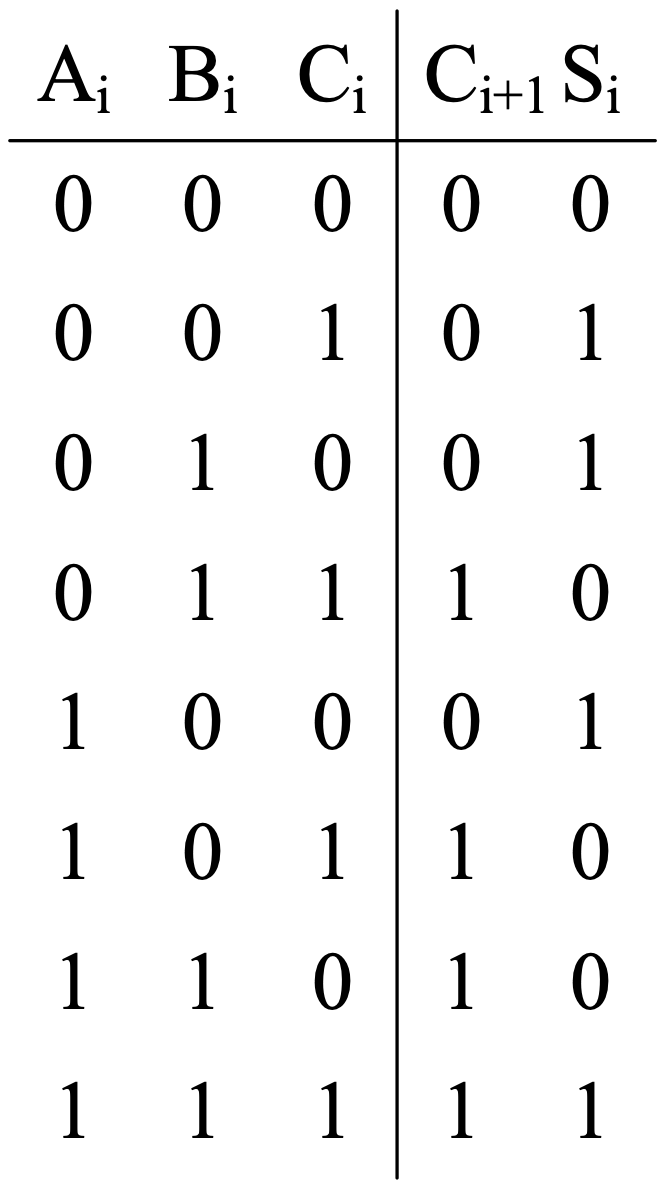
\includegraphics[width=4cm]{./image/全加器真值表.png}  \\[3cm]
                \item [(4)] 電路圖 \\[.8cm]
                  
\includegraphics[width=7cm]{./image/全加器電路圖.png} \\ [.5cm]
              \normalsize
            \end{description}
            \item 加減法電路 \\
              \begin{description}
                \fontsize{16pt}{20}\selectfont
                  \item [(1)] 加法器: $X + Y = X +(Y + 0)$
                  \item [(2)] 減法器: $X - Y = X + (-Y) = X + (\bar{Y} + 1)$
                \normalsize  
              \end{description}
        \normalsize
      \end{enumerate}
    \item [二、]實驗結果
      \begin{description}
        \fontsize{20pt}{22pt}\selectfont
        \item 實驗 (四位元無號數加減法器)
          \fontsize{16pt}{19.2pt}\selectfont
            \begin{enumerate}
              \item 利用7483及XOR閘,實作一個四位元加減法器
              \item 將A連接到固定的二進位數字1001, B連接到四個開關. 執行下列運算, 並記錄其輸出總和S及進位輸出C4的值.
            \end{enumerate}
          \normalsize  
        \normalsize
      \end{description}
    \item [三、]問題討論心得
  \normalsize
\end{description}

\end{document}

